\documentclass{article}
\usepackage{url}
\usepackage{amssymb,amsfonts,amsmath,amsthm,mathtools}
\usepackage{adjustbox}
\usepackage{float}
\usepackage{caption}
\usepackage{mdframed}
\usepackage{lmodern}
\usepackage{bm,bbold}
\usepackage{xfrac, nicefrac}
\usepackage{lmodern}
\usepackage{enumitem}
\usepackage[margin=60pt]{geometry}
\pdfinclusioncopyfonts=1
\captionsetup{width=0.85\textwidth}
\renewcommand{\baselinestretch}{1.5}

\include{notations}
\begin{document}
	\title{Substitution rate responses to changes in effective population size.}
	\author{T. Latrille, N. Lartillot}
	\maketitle
	
	\abstract{
		The quasi-neutral theory of evolution asserts that the effective population size ($\Ne$) plays an important role in shaping the evolution of molecular sequences.
		One consequence is that $\Ne$ modulates selection, such populations with high $\Ne$ would have stronger purifying selection, due to the decrease of random drift.
		In molecular sequence, this effect translates in the decrease in the substitution rate of selected mutations relative to the substitution rate of neutral mutation ($\omega$) with respect to $\Ne$.
		Such theoretical prediction had been observed in empirical data across many clades.
		However, several studies failed to observe such response of $\omega$ to changes in $\Ne$, or with weak strength or direction.
		Computational models of protein folding have observed that $\omega$ can be independent of $\Ne$, which can mathematically be proven under certain assumptions.
		Moreover, non-equilibrium properties can imply that an increase of $\Ne$ can result first in an increase of $\omega$ and then a decrease.
		Together, assumptions about the mapping of sequence to fitness can display a variety of behaviors in the $\omega$ responses to changes in $\Ne$.
		Our goal in this present work is to provide theoretical tools to derive the relationship between $\Ne$ and $\omega$ in the context of a genotype-phenotype-fitness map.
		We derive general formulas, and specify an application in the case of fitness proportional to the probability of protein folding.
		Our compact theoretical results are supported by more complex simulations using 3d structure of proteins.
		We assert that models based on the probability of folding are at odds with empirically results obtained on the $\Ne$-$\omega$ relationship in population genetic dataset.
		However, our framework applied to the case of non-specific interactions between proteins suits more the empirical data.
		We also stress the importance of epistatic interactions in the $\Ne$-$\omega$ relationship, such that it determines to time to reach a new equilibrium.
	}
	
	\section*{Introduction}
	
	Molecular sequences differ across species due to the particular history of DNA substitutions along their respective lineages.
	These substitutions in molecular sequences are the result of the interplay between evolutionary forces such as mutation, selection and random genetic drift.
	These forces have effects at different levels: mutations are carried by molecular sequence, selection is mediated at the level of individuals, while random genetic drift is a population effect.
	Yet, they jointly contribute to the long-term molecular evolutionary process.
	Thus, the challenge of molecular evolution is to tease out their respective contributions, based on comparative analyses.
	
	One main aspect of this challenge is to correctly evaluate the role of random drift in the long term evolutionary process.
	Population genetics theory implies that the strength of drift, due to the stochastic sampling of mutations, is less pronounced in lineage with large effective population size ($\Ne$), and as a consequence, the purification by selection of weakly deleterious mutations is more effective.
	This fundamental idea is at the core of the nearly-neutral theory of evolution.
	The nearly-neutral theory posits that a substantial fraction of mutations are weakly deleterious.
	As a result, the theory predicts that the substitution rate of selected mutations relative to the neutral substitution rate, called $\omega$, decreases along a lineage with higher $\Ne$ \cite{Ohta1972, Ohta1992}.
	
	This prediction has been more quantitatively examined under the assumption that the selective effects of mutations are drawn from a fixed distribution of fitness effects (DFE) \cite{Kimura1979, Welch2008}.
	Assuming a gamma DFE, a key result obtained in this context is an approximate allometric scaling of $\omega$ as a function of $\Ne$ (i.e. $\omega \sim \Ne^{-\beta}$), where $\beta$ is the shape parameter of the DFE.
	In practice, DFEs are strongly leptokurtic, thus predicts a weak negative relation between $\omega$ and $\Ne$.
	
	The substitution rate of selected mutations relative to neutral substitution rate ($\omega$) is an observable quantity of the molecular evolutionary process, at least if we can separately estimate the rate of neutral and selected mutations in a phylogenetic or comparative context.
	Practically, in the case of protein-coding DNA sequences, and assuming that synonymous mutations are neutral, while those selected mutations are the non-synonymous changes affecting the amino-acid sequence, $\omega$ can be identified with the ratio of non-synonymous over synonymous substitution rates ($dN/dS$).
	Thus, in practice, the nearly-neutral argument translates into a predicted decrease in $\omega = dN/dS$ as a function of long-term changes in $\Ne$.
	
	The context of protein coding sequences fostered another modeling approach, based on genotype-fitness map instead of distribution of fitness effects.
	In this alternative approach, the selective effect of a mutation depends on the fitnesses of both source and target amino-acids involved on the mutation \cite{Halpern1998, Rodrigue2010, Tamuri2012}.
	For example, if the target amino-acid has a higher fitness than the current amino-acid, the selective effect of the mutation is positive, and reciprocally negative for a lower fitness.
	Such a modeling approach predicts higher substitution rates between amino-acid with similar biochemical properties.
	More fundamentally, the fitness depends solely on the current genotype, not on the trajectory of mutations leading to this sequence.
	Even though this modeling approach differs substantially from the one assuming a fixed DFE, it also predicts a negative correlation between $\omega$ and $\Ne$ \cite{Spielman2015a, DosReis2015}.
	
	Empirically, variation in $\omega$ along the branches of phylogenetic trees has been inferred using phylogenetic codon models applied to empirical sequences \cite{Yang2001, Zhang2004}. 
	Combining estimations of $\omega$ along branches to life-history traits such as body mass or generation time revealed a positive correlation \cite{Popadin2007, Nikolaev2007}
	Subsequently, integrative inference methods combining molecular sequences and lineage specific quantitative traits have also found that $\omega$ correlates positively with traits such as longevity and body mass \cite{Lartillot2011, Figuet2017}.
	Since longevity and body mass typically correlate negatively with $\Ne$, with low $\Ne$ corresponding to lineage with a large body size and extended longevity \cite{Romiguier2014}, these empirical correlations suggest a negative correlation between $\omega$ and $\Ne$, thus confirming the theoretical prediction of the nearly-neutral theory of evolution.
	However, this correlation between $\omega$ and life-history traits could not be replicated across all experiments, and depending on the clade or the potential biases taken into account, the correlation was found to be either not statistically significant (\cite{Lartillot2012}), or even in the opposite direction \cite{Lanfear2010, Nabholz2013, Weber2014, Figuet2016}.
	
	Mitigated empirical evidence about the response of $\omega$ to changes in $\Ne$ encouraged the search for alternative explanatory mechanisms \cite{Lanfear2014}.
	In this direction, one striking result was the proof that $\omega$ is in fact predicted to be independent of $\Ne$ under very general circumstances, namely, whenever (i) the fitness is a log-concave function of a phenotype and (ii) the phenotype itself is equimutable.
	Equimutability states that the distribution of phenotypic changes due to mutations is independent the current phenotype of the individual \cite{Cherry1998}.
	This general theoretical argument has been invoked in the context of \textit{in silico} experiments of protein sequence evolution, assuming that proteins are under selection for their thermodynamic stability, the fitness being proportional to the folding probability of the protein \cite{Goldstein2013}.
	The thermodynamic stability is itself computed using a 3D structural model of the protein. These simulation experiments have led to the observation that $\omega$ is essentially independent of $\Ne$.
	The explanation proposed for this result is that the distribution of changes in free energy of folding ($\deltadeltaG$) due to mutations is approximately independent of the current free energy ($\deltaG$), thus making the free energy of folding essentially equimutable.
	
	However, the equimutability assumption is a relatively strong one, which also conflicts with simple combinatorial considerations about the relation between sequence and phenotype. For example, if a protein sequence is already maximally stable, only destabilizing (or neutral) mutations can occur. More generally, assuming that the stability of a protein sequence reflects an underlying fraction of positions having already accepted destabilizing amino-acids, then the probability of destabilizing mutational events is in turn expected to directly depend on the current stability of the protein.
	
	In addition, if empirical evidence for a negative correlation of $\omega$ with $\Ne$ is still not totally convincing, another empirical correlation is known to be much more robust, namely, that of $\omega$ with expression level or protein abundance \cite{Duret2000, Rocha2004, Wang2011, Song2017}. Indeed, expression level is one of the best predictors of $\omega$, with highly expressed proteins typically having lower $\omega$ values. Of note, the slope of the response of $\omega$ to changes in expression level is relatively weak \cite{Drummond2005}, although clearly significant. Importantly, many of the theoretical models of protein-coding sequence evolution that have been invoked to explain this correlation between $\omega$ and expression level are such that the response of $\omega$ to changes in expression level or in $\Ne$ should be very similar. Conversely, under strict equimutability, most of these models would predict that $\omega$ should be essentially independent, not just of $\Ne$, but also of expression level, thus at odds with empirical observations.
	
	Overall, there is no doubt that the impact of changes in $\Ne$ (or in expression level) on $\omega$ is at best weak, making empirical estimation more difficult.
	Even if weak, however, an exact theoretical understanding and quantification of how the slope of this relation depends on the underlying map between genotype, phenotype and fitness, would be useful.
	Ultimately, relating proteins structural parameters to the $\omega$-$\Ne$ relationship reveal an intersection between disparate empirical dataset,  coming from protein thermodynamic on one side and comparative genomic on the other side. 
	
	Lastly, the theoretical results discussed so far are all valid only when the balance between mutation, selection and drift is at equilibrium. However, under a model of site-dependent genotype-fitness map, an increase in $\Ne$ first leads to an increase of $\omega$ due to adaptive selection, and subsequently a decrease in $\omega$ due to stronger purifying selection in the long term \cite{Jones2016}.
	Studying only equilibrium properties can thus be misleading. For that reason, the dynamical response of $\omega$ to changes in $\Ne$ must also be addressed, quantified, and its connection with the underlying selective landscape better characterized.
	Dynamical properties of the $\omega$ response to changes of $\Ne$ are of theoretical interest, but are also empirically relevant such that if overlook they could thwart the relation between theoretical expectation and empirical estimates.
	
	% Under the assumption that fitness relates to protein stability, and that such stability if a function of the genotype, the theoretical $\omega$ relationship to $\Ne$ is unknown.
	The goal of this study is to characterize the dynamical and equilibrium response of $\omega$ to changes in $\Ne$, and relate this response to structural parameters of the model.
	To this end, we develop a general mathematical approach for deriving the $\omega$ relationship to $\Ne$ (and expression level) in the context of a given genotype-phenotype-fitness map.
	Based on these results, we discuss the consequences of the assumption that protein stability is a proxy of fitness, and the signatures persisting in DNA sequences observable under such assumption.
	In the light of previously published empirical estimates from protein thermodynamic, and from comparative genomics, we discuss the articulation between empirical data and our mechanistic model.
	We also discuss some of the alternative biophysical mechanisms that could determine the selective landscape on protein-coding sequences, and how they would modulate the slope of the relation between $\omega$ and $\Ne$.
	
	\section*{Results}
	
	\subsection*{Models of evolution}
	
	The results that are presented below are valid for a general category of models of sequence evolution, based on an additive trait $x$ (i.e. such that the coding positions of the sequence contribute additively to the trait), under directional selection specified by a decreasing and log-concave fitness function $f(x)$. As a specific example, we more specifically consider a model of protein evolution under the constraint of thermodynamic stability (See figure \ref{fig:NeChangeInfluence}). This model is inspired from previous work \cite{Williams2006, Goldstein2011, Pollock2012}, except that we make several simplifying assumptions, allowing us to derive analytical equations. 
	%Throughout our derivation, we present the results both for the general case and for the more specific example.
	
	In the original biophysical model, the protein stability is the difference in free energy between folded and unfolded conformations, called $\deltaG$ in kcal/mol.
	Technically, the free energy of the folded are unfolded conformations are computed based on the $3$D conformations of the protein, and using a statistical potential.
	In such models, the stabilizing or destabilizing effect of an amino-acid at a particular site depends on the amino-acids present in the vicinity in $3$D conformation.
	
	We approximate this model such that the destabilizing effect of an amino-acid does not depend on other neighbouring residues.
	Instead, each site contributes independently to $\deltaG$. 
	With such approximation, for each site of the sequence only one amino-acid is stabilizing the protein. 
	All $19$ other amino-acids are equally destabilizing, and each site contribute to an excess of $\gamma > 0$ (in kcal/mol) to $\deltaG$ per destabilizing amino-acids.
	If all amino-acids of the sequence are stabilizing, $\deltaG$ is optimal and equal to $ \alpha < 0$. 
	In this model, the most succinct phenotype of a given genotype (i.e. sequence) is just the proportion of destabilizing amino-acids in the sequence, defined as $0 \leq x \leq 1$. Thus, $\deltaG$ is a linear function of $x$:
	\begin{align}
		\deltaG (x) = \alpha + \Nsite \gamma x,
	\end{align}
	where $\Nsite$ is the number of sites in the sequence. 
	
	For a given $\deltaG$, thermodynamic equations allows to derive the proportion of protein in folded conformation in the cytoplasm, which is assumed to be a proxy for fitness.
	This fitness function is motivated in part that a protein must be folded to perform its function, but can also be justified by the toxic effect of misfolded proteins in the cytoplasm (supp information).
	Analytically, this fitness by the Fermi Dirac distribution and is typically close to $1$, leading to a first-order approximation\cite{Goldstein2011}: 
	\begin{align}
		f(x) = \dfrac{1}{1 + e^{\beta (\alpha + \Nsite \gamma x)}},\\
		\Rightarrow f(x) \simeq 1 - e^{\beta (\alpha + \Nsite \gamma x)}, 
	\end{align}
	where $\alpha$ and $\gamma$ are defined as above, and the parameter $\beta$ is $1.686$ mol/kcal at room temperature.
	
	\subsection*{Susceptibility of $\omega$ to changes in $\Ne$. Analytical approximation}
	
	In this section we present an analytical approximate solution for the response of equilibrium $\omega$ after a change in $\Ne$ (in log space). We call this reponse the susceptibility of $\omega$ to changes in $\Ne$, and denote it as $\chi$:
	\begin{align}
		\chi = \frac{ \der \omega}{\der \ln (\Ne)}
	\end{align}
	Broadly, deriving $\chi$ is done in two steps.
	The first step is to determine the phenotype at equilibrium, when evolutionnary forces of mutation, selection and genetic drift compensate each others.
	Subsequently, differential calculus on the response of the equilibrium phenotype to a change in $\Ne$ allows to ultimately derive an equation for $\chi$.
	The main results are given in the general case of any phenotype-fitness map, and also derived in the specific case where the fitness is proportional to the total amount of folded protein in the specific case of the biophysical model.
	All development are available in Supplementary Materials in the most general case.
	
	First, from a given genotype, mutations changing the sequence have various effect, they can increase or decrease the proportion of destabilizing amino-acid, or do nothing if the mutation is between both destabilizing amino-acids.
	To derive the probabilities of such events to occur, we also make the simplyfing assumption that the transition between amino-acids are equiprobable.
	Altogether, any mutation in the sequence can then have a phenotypic effect of $0$ or $\dx=\sfrac{1}{\Nsite}$, and the probabilities of transition are:
	\begin{gather}
		\begin{cases}
		\dx &\text{ with probability } 1-x, \\
		0 &\text{ with probability } \frac{18 x }{19}, \\
		-\dx &\text{ with probability } \frac{x}{19}.\\
		\end{cases} \label{eq:proba}
	\end{gather}
	In the extreme case of an optimal phenotype ($x = 0$), only destabilization mutations are proposed.
	Moreover, the probability to propose stabilizing mutation (effect $-\dx$), or between destabilizing amino-acids (effect $0$) is proportional to $x$. 
	Or in other words, the mutation bias is proportional to $(1-x)/x$, which this is fundamentally a combinatorial effect, due to the number of mutational opportunities available in either direction.
	
	Second, we need to determine the strength of selection acting on mutations.
	Destabilizing mutations are selected against with a negative selection coefficient which can be approximated by:
	\begin{align}
		s & \simeq \frac{1}{\Nsite}\frac{ \partial \ln f(x) }{\partial x} \label{eq:s} \\
		\Rightarrow s & \simeq - \beta \gamma e^{\beta (\alpha + \Nsite \gamma x)}. \label{eq:s-unfolded}
	\end{align}
	Conversely, stabilizing mutations will be under positive selection with opposite sign but same absolute value.
	It is important to realize that the selective effect is dependent on $x$, and that because fitnesses are log-concave, the absolute value of $s$ increases with regards to $x$.
	
	Based on these expressions for mutational and selective pressure, one can study the evolutionary process unfurls.
	Starting from an optimal sequence, mostly destabilizing mutations will occur, which will reach fixation and accumulate until the selection coefficient against new deleterious mutations is too strong, at which point the protein will reach a point of equilibrium called marginal stability.
	Most importantly the probability of fixation of mutations is affected by genetic drift, parameterized by effective population size ($\Ne$).
	Altogether, at the equilibrium between mutation, selection and drift, the selection coefficient of new advantageous and deleterious mutations reaching fixations are expected to be null on average \cite{Goldstein2013}.
	Formally, and after simplification, the equilibrium phenotype denoted $x\eq$ is given by the equation:
	\begin{align}
		\ln \left( \frac{1 - x\eq}{x\eq} \right) + \ln (19) & \simeq - \frac{4\Ne}{\Nsite} \frac{ \partial \ln f(x\eq) }{\partial {x\eq}} \text{ in the general case,} \\
		\Rightarrow \ln \left( \frac{1 - x\eq}{x\eq} \right) + \ln (19) & \simeq 4\Ne \beta \gamma e^{\beta (\alpha + \Nsite \gamma x\eq)} \text{,} \label{eq:equilibrium}
	\end{align}
	in the more specific case of the biophysical model. This equation essentially expresses the mutation-selection equilibrium: the left-hand side of the equation is the log of the mutation bias at $x$, while the right-hand side is simply $4 \Ne s$.
	
	This equation cannot be solved explicitly for $x\eq$, but an intuition on the consequences of change in $\Ne$ to the equilibirum phenotype $x\eq$ is given in figure \ref{fig:NeChangeInfluence}B.
	Mutation bias decreases weakly with $x$ (blue curve on figure) while the strength of selection increases sharply with $x$.
	The equilibrium phenotype is obtain at their intersection (eq \ref{eq:equilibrium}).
	An increase in $\Ne$ leads to shifting the selective response upward, which then results in a leftward shift of the equilbrium phenotype. 
	The amount of change on $x\eq$, however, is very small if the selection coefficient curve is very steep around the equilibrium set point.
	Of note, the phenotype is not equimutable, meaning the mutational bias is not constant, but nearly so since the derivative of the mutational bias is greatly lower than the derivative of the selection coefficient around the equilibrium point.
	
	\begin{figure*}[htb!]
		\begin{mdframed}
			\centering
			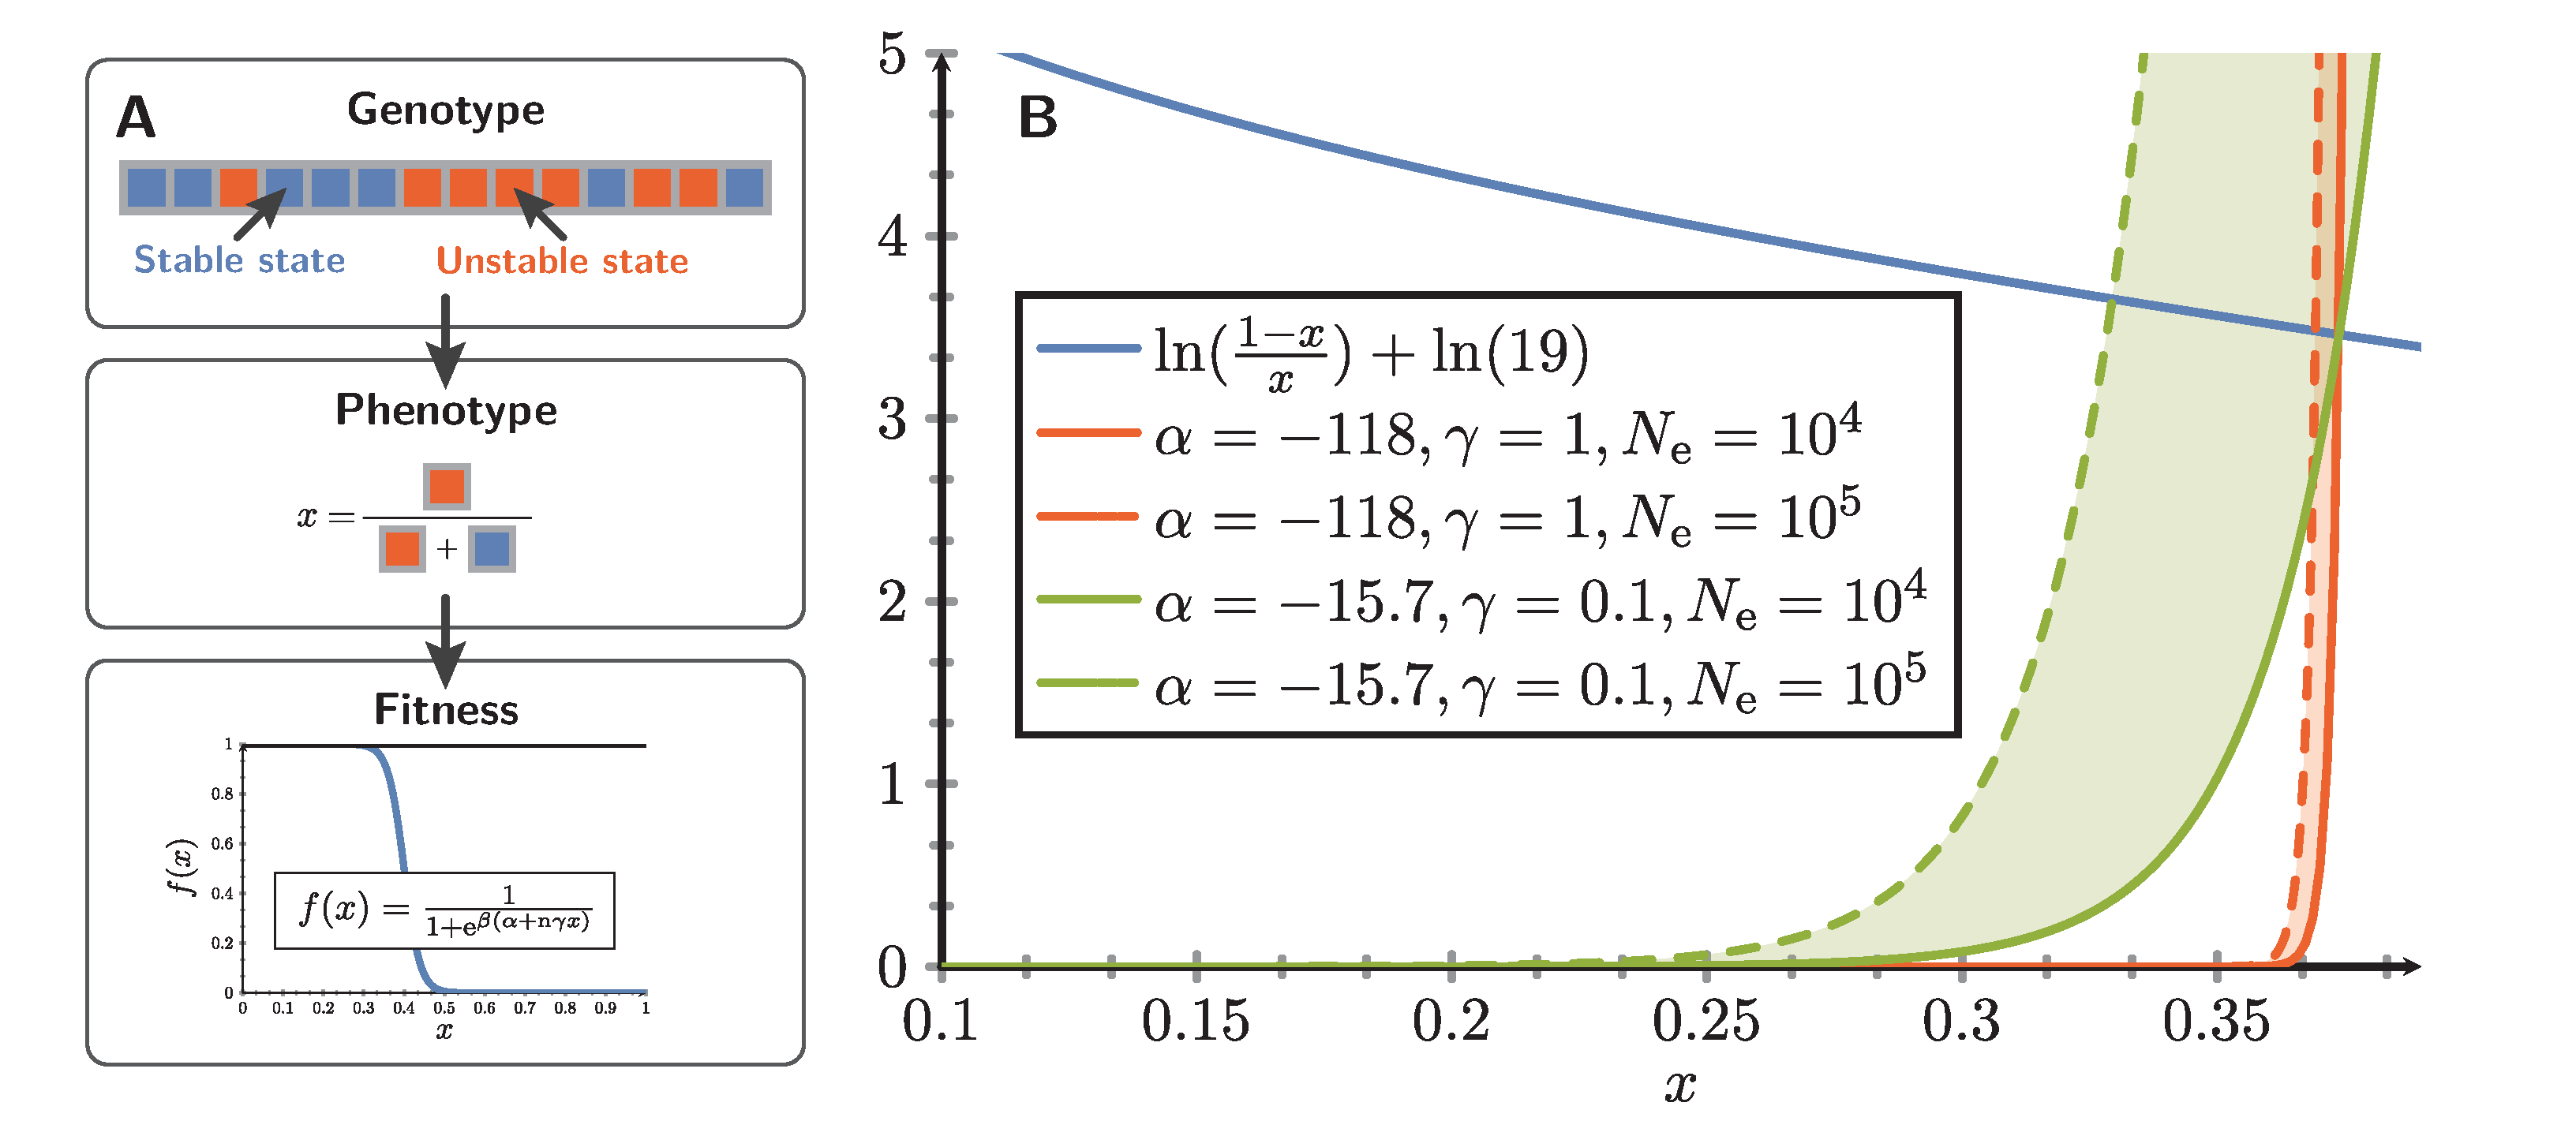
\includegraphics[width=0.9\textwidth, page=1] {artworks/theoretical.pdf}
			\caption{
				\textbf{Theoretical model.}
				Panel A. Illustration of the Genotype-phenotype-fitness map. The phenotype ($x$) is a real-valued summary of the genotype, and is defined in our model as the fraction of destabilizing sites in the sequence. The fitness is a decreasing log-concave function of the phenotype.
				Panel B. Illustration of the $\omega$ susceptibility after a change in $\Ne$. The equilibrium $x\eq$ is determined by the equation $\ln(\frac{1 - x\eq}{x\eq}) + \ln(19)=4\Ne \beta \gamma e^{\beta (\alpha + \Nsite \gamma x\eq)}$. The right-hand side of the equation increases exponentially with $x$ where $\Nsite \gamma$ is the exponential growth rate. Thus when $\Nsite \gamma$ is large (red solid line), increasing $\Ne$ (red dotted line) only changes subtly $x\eq$ (x-axis of the crossing with the blue solid line). On the other hand, when $\Nsite \gamma$ is low (green solid line), increasing $\Ne$ (green dotted line) involve a stronger response of $x\eq$. Moreover, changes in $x\eq$ reflects the changes in $\omega$ since both are related by a monotonous function (equation \ref{eq:dnds}). The value of $\alpha$ has been chosen given all other parameters such that the solid lines all cross at the same point.
			}
			\label{fig:NeChangeInfluence}
		\end{mdframed}
	\end{figure*}
	
	The argument thus far explains how $x\eq$ varies with $\Ne$.
	To capture how $\omega$ varies with $\Ne$, we also need to obtain an expression for $\omega$ as a function of $x\eq$. 
	At equilibrium we can derive the expected substitution rate of mutations changing the amino-acid sequence, and by normalizying by the substitution rate of neutral mutations, $\omega$ simply approximates to:
	\begin{gather}
		\omega \simeq x\eq \label{eq:dnds}
	\end{gather}
	This simple approximation is due to substitutions at destabilizing sites (proportion $x\eq$) to one of the other destabilizing amino-acids, which are effectively neutral and compose the largest proportion of proposed mutations with substantial probability of fixation (see equation \ref{eq:proba}).
	
	Finally, $x\eq$ at equilibrium (eq \ref{eq:equilibrium}) is implicitly a function of $\Ne$ and the other parameters.
	Implicit derivation of the equilibrium with regards to $\Ne$ (see supp info) allows the derive the response of $x\eq$ and ultimately $\omega$ after a change in $\Ne$.
	After simplifications, the susceptibility of $\omega$ to changes in $\Ne$ can be approximated in terms of a very compact equation for the general case: 
	\begin{gather}
		\chi = \frac{ \der \omega}{\der \ln (\Ne)} \simeq - \frac{\frac{ \partial \ln f(x\eq) }{\partial {x\eq}}}{\frac{ \partial^2 \ln f(x\eq) }{\partial {x\eq}^2}}
	\end{gather}
	The susceptibility is thus equal to the inverse of the relative curvature, i.e. the ratio of the second to the first derivatives, of the log-fitness function, taken at the equilibrium phenotype. Of note, this susceptibility is strictly negative for decreasing log-concave fitness functions, asserting that $\omega$ is a decreasing function of $\Ne$. In addition, the susceptibility itself is low (i.e. $\omega$ responds more weakly) for strongly concave log-fitness functions, thus formally capturing the intuitive argument developed above (figure \ref{fig:NeChangeInfluence}B).
	
	In the specific case of the biophysical model, the susceptibility ($\chi$) simplify to:
	\begin{gather}
		\chi \simeq -\dfrac{1}{\beta \Nsite \gamma}, 
	\end{gather}
	Meaning that $\omega$ is linearly decreasing with $\Ne$ in log scale, since $\chi$ is independent of $x\eq$ and thus the exact value of the equilibrium phenotype has no impact on the slope.
	Moreover, only the compound parameter $\beta \gamma \Nsite$ has an impact on the slope of the linear relationship.
	In practice, $\gamma = \Delta \Delta G$ determine the slope of the linear relationship between $\omega$ and $\Ne$, while $\alpha = \Delta G_{\text{min}}$ can never obtained solely from this slope.
	Importantly, only empirical relative values of $\Ne$ (multiplicative) and $\omega$ (additive) are sufficient to estimate $\chi$, absolute values are not necessary to estimate the slope.
	Conversely, if one seek to determines $\Delta G_{\text{min}}$, one need the intercept of the linear relationship, and thus absolute value of $\omega$ and $\Ne$ are necessary.
	% Although the general equation seems to suggest in appearance that elasticity only depends on the fitness function, in fact, what the biophysical model shows is that the elasticity can actually be modulated in two ways: by playing on the genotype / phenotype relationship (here, $\gamma$), or by playing on the fitness phenotype relationship (here, beta). All the more reason to consider beta as a potentially free parameter too.
	
	Other parametrization of the fitness function shed light on the robustness of the theoretical results.
	If the selective coefficient itself is not equal (equation \ref{eq:s-unfolded}) but proportional to the total amount of misfolded protein, and the expression level of the protein is denoted $A$, then the response of $\omega$ to changes in $\Ne$ is the same as the response to changes in $A$ (supplementary materials):
	\begin{align}
	s & \propto - \beta \gamma y e^{\beta(\alpha + \gamma \Nsite x)} \\
	\Rightarrow \chi \frac{ \der \omega}{\der \ln (\Ne)} = \frac{ \der \omega}{\der \ln (A)} & \simeq -\dfrac{1}{\beta \Nsite \gamma}.
	\end{align}
	Meaning we should observe the same relationship between $\omega$ and either effective population size ($\Ne$) or expression level ($A$).
	
	Under empirically relevant value of $\Nsite=300$ sites and $\gamma=1.0$ kcal/mol \cite{Zeldovich2007}, the susceptibility $\chi \simeq -0.002$.
	In other words, for a increase in $\Ne$ of $6$ orders of magnitude, $\omega$ decrease approximately of $0.01$, a subtle relationship that requires laborious effort to be detected in simulated data, and large amount of empirical data with few bias and noise to be detectable. In addition, it would imply an equally weak relation between $\omega$ and expression level.
	
	\subsection*{Simulation experiments}
	
	Our theoretical derivation of the susceptibility of $\omega$ to changes in $\Ne$ is based on several simplifying assumptions about the evolutionary model and makes multiple approximations. In order to test the robustness of our main result, we therefore conducted systematic simulation experiments, relaxing several of these assumptions. In each case, simulations were conducted under a broad range of values of $\Ne$, monitoring the average $\omega$ observed at equilibrium and plotting the scaling of these measured equilibrium $\omega$ as a function of $\Ne$. 
	
	Specifically, with respect to mutations, our derivation assumes that all amino-acids transition are equiprobable, in other word the complexity of the genetic code is not taken into account.
	Simulating evolution of DNA sequence, and taking into account a matrix a mutation rate between nucleotide allow to test directly the robustness of the results to this assumption.
	Furthermore, with regards to the phenotypic effects of amino-acid changes, we assumed that all destabilizing amino-acids are have an identical impact on protein stability.
	In reality, one would expect conservative amino-acid replacements to be less destabilizing than radical changes.
	This assumption is relaxed in our simulation, indeed destabilizing effects in each position, instead of being identical for all alternative amino-acids, are now proportional to the Grantham distance \cite{Grantham1974} between the optimal amino-acid in this position and the amino-acid proposed by the non-synonymous mutation.
	Finally, the number of sites in the sequence ($\Nsite$) is assumed to be large such that the selection coefficient is well approximated by the fitness derivative (equation \ref{eq:s}).
	The robustness of such approximation is test in the simulations with sequences of a finite number of sites ($\Nsite=300$).
	
	Simulations demonstrate that the relation between $\omega$ and log-$\Ne$ is indeed linear, at least in the range explored here, and that the slope of the linear regression matches the expected theoretical value (figure \ref{fig:GoldsteinVsToy}A).
	Secondly we observe that the parameter $\alpha$ has virtually no effect on the slope of the linear regression, as expected also theoretically (figure \ref{fig:GoldsteinVsToy}B). Instead, decreasing $\alpha$ (to more negative values) merely results in an overall increase in $\omega$ over the whole range of $\Ne$ (i.e. has an impact on the intercept, not on the slope). This is due to the fact that decreasing $\alpha$ shifts the equilibrium to higher $x\eq$, since more destabilizing sites can then reach fixation before reaching the point of marginal stability.
	
	Finally, we relaxed our assumption that each site of the sequence contribute independently to $\deltaG$, by taking into account the $3$D structure of protein and using a statistical potential to estimate $\deltaG$.
	We implemented the original model \cite{Williams2006, Goldstein2011, Pollock2012}, in which the free energy of the folded are unfolded conformations are computed using $3$D structures of the protein conformations and pairwise contact potential energies between neighboring amino-acid residues \cite{Miyazawa1985} (see Supplementary Materials).
	The original works showed that under such $3$D model $\omega$ is approximately independent of $\Ne$ \cite{Goldstein2013}.
	Using extensive simulations in order to obtain sufficient resolution, we observe that $\omega$ is in fact weakly dependent on $\Ne$, being approximately linear with log-$\Ne$ (figure \ref{fig:GoldsteinVsToy}C).
	Moreover, the observed slope matches the theoretical value considering $\deltadeltaG = 1.0$ kcal/mol for destabilizing mutations and $\Nsite=300$. 
	In such experiment, $\alpha=-118$ kcal/mol as it is the $\deltaG$ of the optimal sequence of $300$ sites \cite{Goldstein2011} (figure \ref{fig:GoldsteinVsToy}D).
	\begin{figure*}[htb!]
		\begin{mdframed}
			\centering
			\includegraphics[width=0.9\textwidth] {artworks/Elasticity.png}
			\caption{
				\textbf{$\bm{\omega}$ susceptibility to change in $\bm{\Ne}$}.
				For each population size, $100$ simulations were performed and the average (solid line) and $90\%$ confidence interval (shaded area) are shown.
				Panel A. The fixed parameters are $\gamma=1$, $\Nsite=300$, $\beta=1.686$, and for each non-optimal amino-acid, $\gamma$ is scaled by the Grantham distance to the optimal amino-acid. $\alpha$ are given in the legend. Decreasing $\alpha$ (to more negative values) increases $\omega$ but changes hardly the slope of the linear regression, as expected theoretically.
				$\omega$ at equilibrium as a function of $\bm{\Ne}$ (log scale).
				Panel B. The fixed parameters are $\Nsite=300$ and $\beta=1.686$. Parameters $\alpha$ and $\gamma$ are given in the legend.
				$\gamma$ is increased and $\alpha$ is changed accordingly such that the equilibrium value $x\eq$ is kept constant, by solving numerically equation \ref{eq:equilibrium}.
				The slope of $\omega$-$\Ne$ relationship decreases proportionally to the inverse of $\gamma$, as predicted by our theoretical model.
				Panel C. In the model of 3D free energy of folding, $\omega$ at equilibrium is weakly dependent on log-$\Ne$, but not completely as originally claimed \cite{Goldstein2013}.
				This weak dependence matches the theoretical prediction of our additive free energy model that the linear relation (dashed line) has a slope equal to $(\beta \Nsite \gamma)^{-1} = 0.00198 \simeq 0.00124$.
				Bottom D, the fixed parameters are $\alpha=-118$, $\gamma=1$, $\Nsite=300$, $\beta=1.686$, and for each non-optimal amino-acid, $\gamma$ is scaled by the Grantham distance to the optimal amino-acid.
				Moreover, with the Grantham model, the $\omega$ matches the empirical 3D model of Golstein \& Pollock and the theoretical prediction.
				\label{fig:GoldsteinVsToy}
			}
		\end{mdframed}
	\end{figure*}
	\subsection*{Epistasis and time to relaxation}
	Although the equilibrium value of $\omega$ after changes in $\Ne$ is an important feature of the $\omega$-$\Ne$ relationship, another characteristic that is scarcely studied is the dynamic aspect, particularly the relaxation time to reach the new equilibrium $\omega$ \cite{Jones2016}.
	We observed in our simulations that the determining factor of the relaxation time is the number of sites $\Nsite$ (figure \ref{fig:relaxStability}A).
	These observations match the theoretical prediction that high epistasis leads to faster return to equilibrium, since more mutational opportunities are available for driving the trait closer to equilibrium.
	
	It may be useful to compare the relaxation pattern observed here with the predictions under two alternative models of sequence evolution, representing two extreme scenarios. On one side, under a site-independent fitness landscape, such as those contemplated by many current mutation-selection models \cite{Halpern1998, Rodrigue2010}], thus with no epistasis, every site has to adapt on its own to the new change in $\Ne$. As a result, the relaxation time is vey long, of the order of the inverse of the per-site substitution rate. 	
	On the other side, assuming a fixed distribution of fitness effect (DFE), the response of $\omega$ is instantaneous (figure \ref{fig:relaxStability}B).
	
	Disregarding simulations under a fixed DFE, another characteristic observed is the non-continuity of $\omega$ after a change in $\Ne$.
	Both an increase and decrease in $\Ne$ lead to a discontinuity in $\omega$.
	Most importantly, $\omega$ is suddenly higher regardless of the change's direction in $\Ne$, then smoothly reaching the equilibrium value (figure \ref{fig:relaxStability}A \& \ref{fig:relaxStability}B).
	The similarities in these non-equilibrium properties can both be explained mechanistically.
	Under low $\Ne$ (between $0$ and $100$ My in the simulation), the phenotype is far away from the optimal phenotype and loosely constrained because the strength of selection is weaker.
	The reaction to an increase in $\Ne$ (at $100$ My in the simulation) is first a higher constrain and a traction toward a more optimal phenotype, which translate into suddenly higher $\omega$.
	Conversely, under high $\Ne$ (between $100$ and $400$ My in the simulation) the phenotype is closer to optimal and tightly constrained.
	The reaction to a decrease in $\Ne$ is first a lower constrain and thus a $\omega$ closer to the neutral case, which translate into higher $\omega$.
	To note, an increase in $\Ne$ can theoretically and possibly lead to a temporarily $\omega > 1$ due to adaptive evolution \cite{Jones2016}, while an decrease in $\Ne$ always imply $\omega < 1$ due to at most a neutral regime of relaxed selection.
	
	\begin{figure*}[htb!]
		\begin{mdframed}
			\centering
			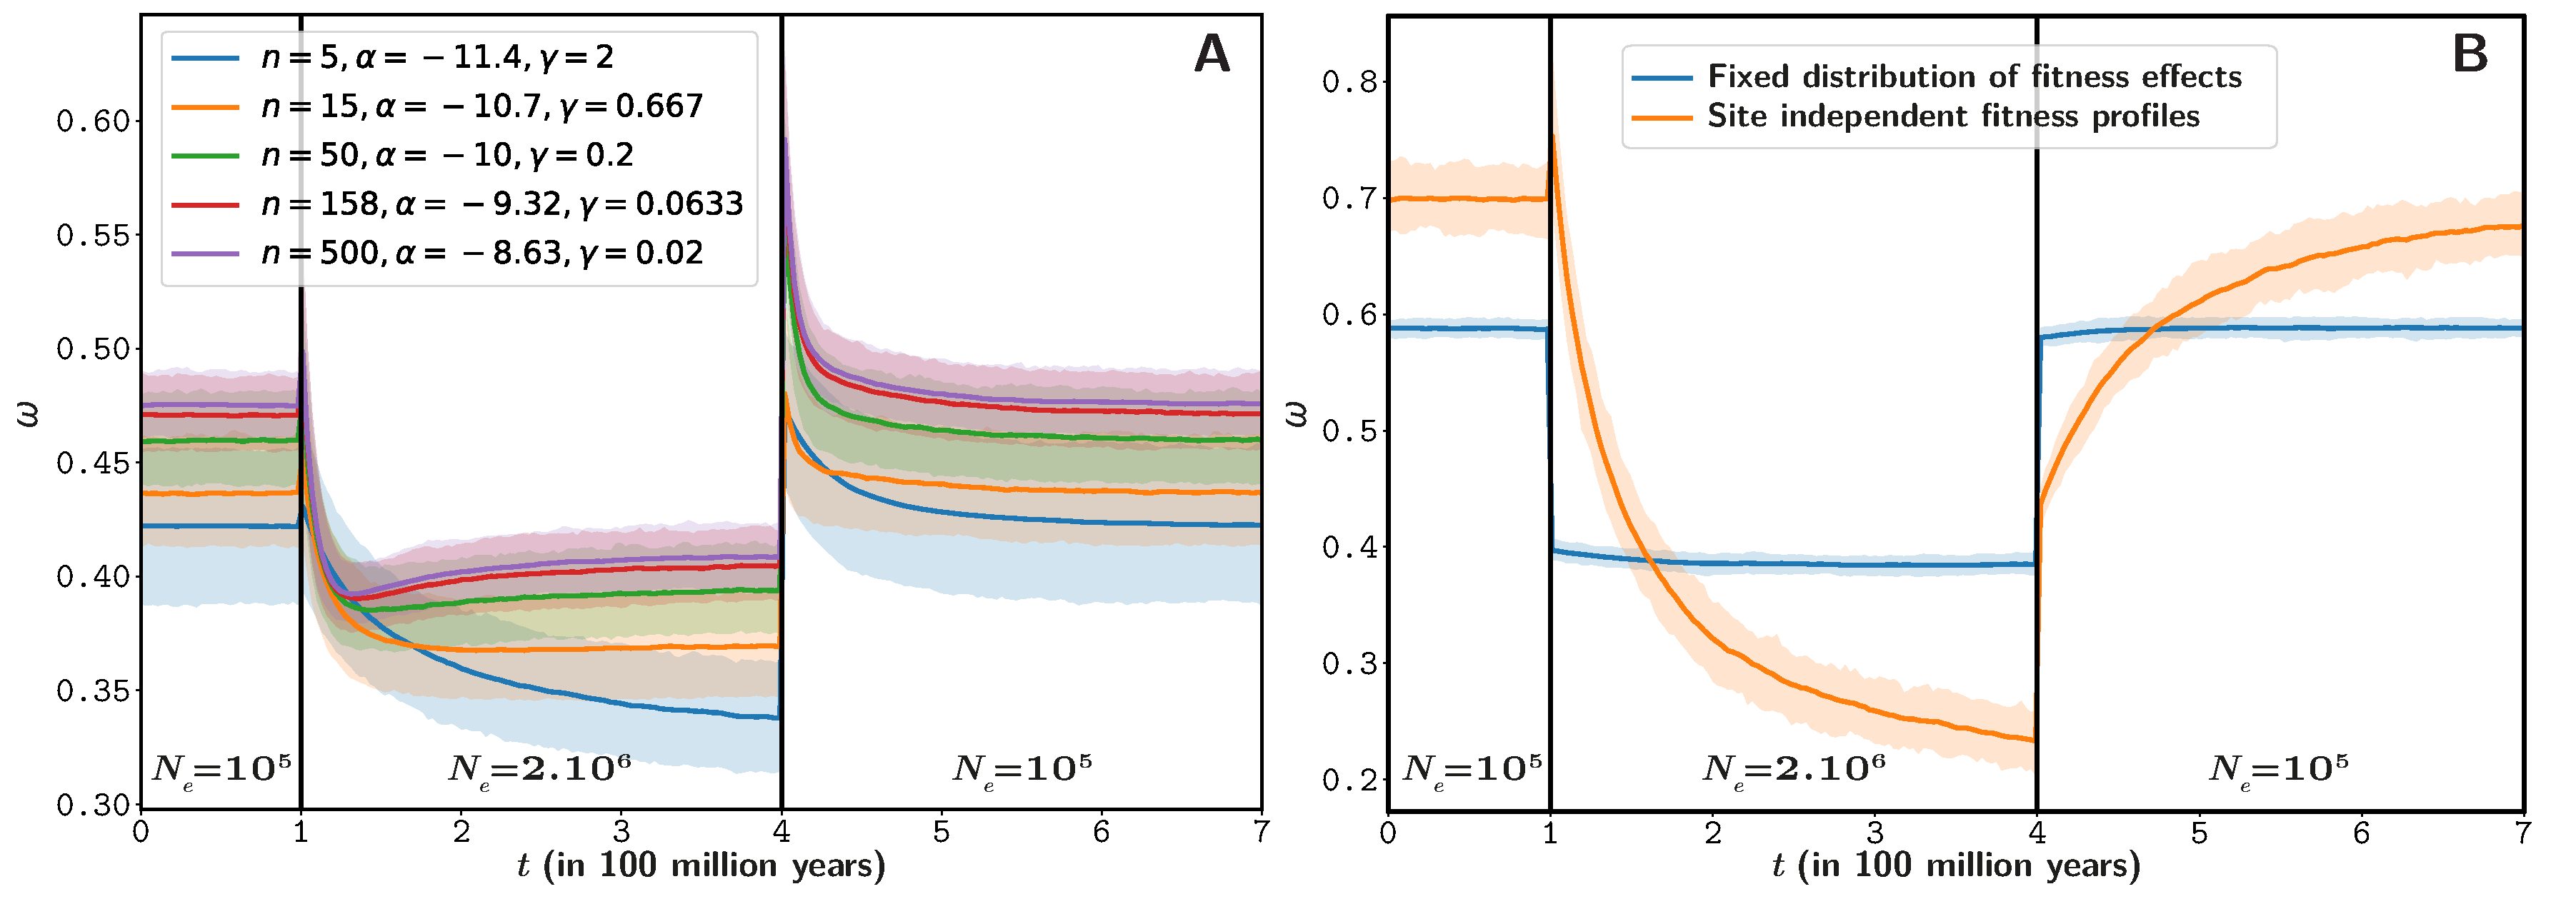
\includegraphics[width=0.9\textwidth] {artworks/Relaxation.pdf}
			\caption{
				\textbf{$\bm{\omega}$ relaxation after a change in $\bm{\Ne}$}.
				Solid line corresponds to the average over $1000$ replicates and the shaded area correspond to the $90\%$ interval among replicates. 
				The mutation rate ($\mu$) is $1e{-8}$ per year per site, and the total time of the computation is $700$ million years.
				Panel A. 
				$\beta=1.686$ for all simulations.
				The DNA sequence of $500$ sites is divided into exons of equal size.
				However the number of sites per exon changes between simulations from $\Nsite=5$ to $\Nsite=500$.
				Moreover, $\gamma$ is changed according to the exon size such that the product is kept constant, thus the susceptibility of the $\omega$ to changes in $\Ne$ is kept constant.
				Finally, $\alpha$ is changed accordingly such that the equilibrium value $x\eq$ is kept constant, by solving numerically equation \ref{eq:equilibrium}.
				As such, whatever the exon size, $x\eq$ and $\chi$ are kept constant and thus the observed effect is due to the number of sites in the exon.
				We observe that increasing the number of sites implies a reduced time to reach the new equilibrium.
				Panel B. In context of a fixed fitness landscape, where each amino-acid has different fitness (site-specific profile), the time taken to reach the new equilibrium value of $\omega$ after a change in $\Ne$ is long, such that relaxation rate is on the order of the mutation rate. In the context of a distribution of fitness effects (DFE), the relaxation time is non-existent and the new equilibrium value of $\omega$ is reached instantaneously.
			}
			\label{fig:relaxStability}
		\end{mdframed}
	\end{figure*}
		
	
	\section*{Discussion}
	% Goal and theoretical results
	The negative relationship between the relative substitution rate of selected mutations ($\omega$) and the effective population size ($\Ne$) has been predicted theoretically under the quasi-neutral theory of evolution.
	Empirical data showed mitigated confirmation of this prediction, encouraging alternative explanatory mechanism.
	One such explanation, developed in the context of genotype-phenotype-fitness map, demonstrated the absence of $\omega$ susceptibility to changes in $\Ne$ if the probabilities of phenotype changes are invariant to the current phenotype.
	We argue that this assumption can be relaxed, and provide theoretical tools to derive the relationship between $\omega$ and $\Ne$ at equilibrium in this context.
	We apply our framework in the special case of fitness proportional to the proportion of folded proteins. 
	Our theoretical results demonstrate that the relationship between $\omega$ and $\Ne$ (in log space) is linear with a negative slope.
	This slope is a function of structural parameters of the protein, and is inversely proportional to the product of the sequence size and the average change in conformational energy of destabilizing mutations, leading in practice to a very subtle and weak relationship. 


	Our compact theoretical results are supported by more complex simulations of protein evolution relaxing several assumptions.
	Particularly, our theoretical prediction match a numerical model of protein evolution, in which the free energy of the folded are unfolded conformations are computed using $3$D structures of the protein conformations.
	Previous studies using this model presented an apparent lack of $\omega$ susceptibility to changes in $\Ne$ \cite{Goldstein2013}.
	We argue the apparent lack of susceptibility is in fact due to the subtle relation, and require extensive computation to be detected.
	
	\subsection*{Empirical relevance}

	% Our theoretical results are robsut to approximations
	% Goldstein \& Pollock model don't have a null susceptibility
	Based on empirical estimate of the structural parameters ($\beta = 1.686,\ \gamma=1, \Nsite=300$), the slope of the linear relationship between $\omega$ and log-$\Ne$ would be $\chi \simeq -0.002$.
	Empirically, inference of the $\omega$ susceptibility in Primates, using both polymorphism and divergence data estimated $\chi \simeq X$, approximately $X$ times greater than our theoretical prediction \cite{Brevet2019}.
	More empirical data across different clades would be required to robustly consolidate such empirical observation.
	However, in the light of empirical data tending to demonstrate negative relationship between $\omega$ and $\Ne$, models based on the probability of folding are not sufficient to explain the observation of such stastically significant relationship.
	% Our result show the fitness proportional to proportion of folded folding is at odd with empirical data
	
	% Stress the importance that susceptibility is valid for Ne and protein abondance
	Furthermore, our theoretical results demonstrate that the relationship between $\Ne$ and $\omega$ is the qualitatively and quantitatively the same as between protein abundance and $\omega$, whenever protein fitness is determined by the deleterious effect of unfolded proteins.
	As such, dataset relating $\omega$ to either $\Ne$ or protein expression could in principle be used to determine whether the slope is the same.
	However such endeavor is easily prone to biases and confounding factor, due to study across different clades and across different genes.
	
	% Protein-protein interactions
	Notably, our theoretical approximations apply more broadly to protein-protein interactions (using a mean-field argument, supplementary materials), where protein may either be in free form or engaged in a non-specific interactions with other proteins. 
	In non-specific interactions, stabilizing amino-acids at the protein surface are hydrophilic and destabilizing amino-acid are hydrophobic (sticking to  hydrophobic residues in other proteins).
	Fitting this model with empirical structural estimates \cite{Zhang2008}, we obtain an susceptibility of $\chi \simeq -0.2$ thus a much stronger response than under the model based on conformational stability.
	This effect is due to less sites in the protein being involved in protein-protein interaction than for conformational stability, in addition to the lower energy engaged in the contacts.
	Comprehensively, the assumption that protein fitness is in part determined such as to avoid non-specific interaction leads to a stronger response of $\omega$ to changes in $\Ne$, is more compatible with empirical data obtained in comparative genomics.
	% Such path might worth be explored !
	
	Finally, an integrative inference framework of comparative genomics parameterized by structural parameter, expression level and effective population size can in principle allow to robustly test our prediction with empirical data. 
	Orthogonally, this inference framework could allow to estimate unknown variable, for example ancestral effective population size, with enough signal and calibration of the other parameters. 
	Such inference framework should be careful with some caveats that we will subsequently discuss.
	\subsection*{Inference models}
	% Categories of models
	Models of inference are classified broadly into phenomenological and mechanistics.
	Mechanistic models dissect the causation chains and construct model for first-principles, while phenomonological models aims to determine the statistical significativity of parameters.
	
	% Phenomenological models
	An example of such phenomenological model are the models parametrized directly in $\omega = dN/dS$.
	They will for example tell us which branch of the tree, or which site of the sequence has a decrease or increase in $\omega$ but not the underlying reason for such changes, which can be either mutation, selection, drift or another evolutionary force.
	For example, in such models, a mutation and its reverse mutation do not have opposite selection coefficient.
	As such they can not disentangle the potentially confounding effect of mutation, selection and drift.
	Neither can they predict the nature of the functional relationship between population genetics or structural physico-chemical parameters to $\omega$.
	As such, of mechanistic models are necessary to construct an integrative comparative framework.
	
	% Site specific mechanistic models of evolution 
	On the other hand, mechanistic models of evolution mapping genotype to fitness have so far assumed site-independent fitness map, mainly for computational rationals.
	Previous studies have argued that model of protein evolution should consider epistasis for various empirical reasons such as rate heterogeneity along the sequence, rate and time dependence of convergence, role of compensatory substitutions \cite{Goldstein2017}.
	We argue that epistasis also has an important role in the response of $\omega$ to changes in $\Ne$, both in terms of susceptibility and dynamic of the response.
	Fundamentally, we argue that any site-specific model implies a slow dynamic and a strong susceptibility, and adding epistasis to the model imply a faster dynamic and a weaker susceptibility.
	Intuitively, this effect originate that each site is to adapt independently to changes in $\Ne$ leading to overall a slow response (substitutions must  affect all sites), and a strong susceptibility since each site will change its position in the fitness landscape.
	Taking into account epistasis, the burden of adapting to changes in $\Ne$ is shared by more sites, such that all of them don't have to adapt. 
	As a conclusion, both mechanistic and phenomenological models of inference are at risk to endure some culprits.
	In retrospect, these pitfalls have been anticipated thanks to the intuitions developed in the construction of this mechanistic genotype-phenotype-fitness model.
	
	\subsection*{Theoretical modeling}
	% Analogy to physics
	This study elaborate the signature on DNA sequences of a long-term evolutionary process as emergent from population-genetics and structural physico-chemical first principles.
	Hence, physico-chemical vocabulary and theory are recruited to describe the molecular details.
	More widely, our modeling is imprinted with vocabulary and analogy to physical systems, with wording in the likes of forces, susceptibility and dynamic.
	We argue analogy between evolutionary and mechanstic system is not restricted to wording, but allows to visualize and intuit of the causality chains and which approximation can be made such as to derive analytical tractable results.
	Because it is constructive approach, and not solely intuitive, the robustness of theoretical results to approximations can be asserted by computational implementation. 
	Computational models offers a means to test the validity and robustness, while the mathematical models offers an intuitive mechanistic mental analogy.
	
	% Mechanical analogy
	% Elasticity with springs ? Surface tension with molecule and radius of the 
	% Elasticity ? Susceptibility (dimensionless) ? Compliance (units of metres per newton) ? Flexibility (units of metres per newton) ? 
	In the mechanical analogy, the phenotype represent a spatial coordinate of the system, which is determined by external evolutionary forces; namely mutation, selection and drift.
	These evolutionary forces are homologous to springs attached and stretching the phenotype in various directions and with various intensity, and the aim is to find the equilibrium point.
	Once the equilibrium point is determined, the deformation of the phenotype (called strain) can be studied whenever applying an differential stress to the system.
	Elasticity refers to a reversible deformation of a system upon a external force, hence its ability to return to its original state when that force is removed.
	Intuitively, changing the free energy of the reference phenotype ($\Delta G_{\text{min}} = \alpha$) leads in first approximation to changes in the equilibrium point but not the stiffness of the springs, because only the reference is changed, meaning the elastic coefficient is conserved as found in our theoretical results.
	Conversely, stiffness ot the strings increases with regards to $\Delta \Delta G = \gamma$, meaning a that change in the stress applied to the system ($\Ne$) result in a weak deformation ($\omega$) at the new equilibrium.
	
	% Thermodynamic analogy 
	% Analogy to Clapeyron formula ? TdP/dT = ΔH/ΔV, where T is analogous to Ne
	In the thermodynamic analogy, the phenotype is a macroscopic resultant of microscopic states of each site of the sequence.
	Such example could be homologous to the Ising model, and each site of the sequence is a magnetic dipole which can be up or down (destabilizing or stabilizing).
	The phenotype is an aggregate of the microscopic states, simply the proportion of destabilizing states.
	Under external forces, the macroscopic proportion is statistically determined by the potential energy of the system, and the susceptibility ()analogous to magnetic susceptibility) of the system is the response of macroscopic observable to change in temperature (inverse of $\Ne$).
	
	% Fundation to integrate other forces
	Altogether, this framework can be used as a premise % (groundwork, foundation, starting point,...)
	to integrate other external evolutionnary forces.
	Additional molecular processes could be included, for instance GC-biased gene conversion inducing a bias in the nucleic composition of genomes. 
	The change of equilibrium due to the GC-bias, and the magnitude of the response could be investigated, as to describe the signatures observable on molecular sequence, factoring the effect of mutation, selection and drift.
	Finally, we hope the result of this work, and more broadly the framework can foster the understanding of observable signature of a long-term evolutionary process as emergent from ecological parameters and molecular physico-chemical first principles.

	\section*{Materials \& Methods}
	Protein sequence evolution is simulated under an origin-fixation model \cite{McCandlish2014}, where one sequence represent the whole population.
	From the resident DNA sequence $\ci$, we define $\setNeighbors$ as the set of all possible mutant that are one nucleotide away from $\ci$, and were mutant sequences containing a stop codon are excluded.
	For a protein of $\Nsite$ amino-acid sites, $\left| \setNeighbors \right| \leq 9 \Nsite$, since each codon has a maximum of $9$ possible mutant codons that are one mutation away and that are not stop codon.
	For each mutant sequence $\cj \in \setNeighbors$, we compute its fitness and subsequently the selection coefficient of the mutant:
	\begin{equation}
	s \left( \ci,\cj\right) = \dfrac{ f \left(\cj \right) - f \left(\ci\right) }{f\left( \ci \right)}.
	\end{equation}
	The next event of mutant invading the population, and the time to reach such event is chosen using Gillespie algorithm, according to the rates of substitution between sequences:
	\begin{equation}
	\submatrix_{\itoj} = \mu_{\itoj} \dfrac{4 \Ne s \left( \ci,\cj\right)}{1 - \e^{-4 \Ne s \left( \ci,\cj\right)}}, 
	\end{equation}
	where $\mu_{\itoj}$ is the mutation rate between $\ci$ and $\cj$, determined by the underlying $4x4$ nucleotide mutation rate matrix, and ${\submatrix_{\itoj}} = \mu_{\itoj}$ in the case of synonymous substitutions.
	Various optimization are implemented to reduce the computation time of mutant's fitnesses.
	The simulation starts with a burn-in period to reach mutation-selection-drift equilibrium.
	\subsection*{Models of fitness function}
	\label{MatMet:folding}
	Under a simulation of protein folding with an additive model of free energy, the protein's difference in free energy between folded and unfolded state is given by:
	\begin{equation*}
	\deltaG\left(\ci\right) = \alpha + \Nsite \gamma * x\left(\ci\right), 
	\end{equation*}
	where $0 \leq x\left(\ci\right) \leq 1$ is the distance of $\ci$ to the optimal sequence.
	For each site of sequence, the optimal amino-acids are chosen randomly at initialization, and the distance between the current amino-acid and the optimal is scaled by the Grantham amino-acid distance \cite{Grantham1974}.
	Wrightian fitness is defined as the probability of our protein to be in the folded state, given by the Fermi-Dirac distribution: 
	\begin{equation}
	f(\deltaG\left(\ci\right)) = \dfrac{e^{-\beta \deltaG\left(\ci\right) }}{1 + e^{-\beta \deltaG\left(\ci\right) }} = \dfrac{1}{1 + e^{\beta \deltaG\left(\ci\right) }}, 
	\end{equation}
	where $\beta$ is the inverse of the temperature ($\beta=1/kT$).
	
	Under a simulation with site independent fitness profiles, a fitness profile give a fitness for each amino-acid (vector of size $20$).
	Each site of the protein has a specific amino-acid fitness profile.
	Overall, the protein phenotype is computed as the sum of site-specific selection coefficient, obtained by accessing the amino-acid present at each site of the protein.
	The selection coefficient of the mutant $\cj$ is:
	\begin{equation}
	s \left( \ci,\cj\right) = \sum_{1 \leq \site \leq \Nsite} \ln \left( \dfrac{G_{\site} \left(\cj(\site) \right)}{G_{\site} \left(\ci(\site) \right)} \right) ,
	\end{equation}
	where $G_{\site}$ is the fitness profile at site $\site$, obtained in empirical experiment \cite{Bloom2017}.
	
	
	Under simulation with a fixed distribution of fitness effects (DFE), the selection coefficient of the mutant $\cj$ is gamma distributed (shape $\beta > 0$):
	\begin{equation}
	- s \left( \ci,\cj\right) \sim \text{Gamma} \left( \bar{|s|}, \beta \right)
	\end{equation}
	\subsection*{$\bm{\omega}$ along the simulation}
	From the set of mutants $\setNeighbors$ that is one nucleotide away from $\ci$, we define the subsets $\setNonSynNeighbors$ and $\setSynNeighbors$ that are respectively the set of non-synonymous and synonymous mutants, where $\setNonSynNeighbors \cup \setSynNeighbors = \setNeighbors$.
	As in previous works \cite{Spielman2015a, DosReis2015, Jones2016}, the ratio of non-synonymous over synonymous substitution rates of the sequence is defined as :
	\begin{align}
	\omega(t) &= \dfrac{\sum_{\cj \in \setNonSynNeighbors} \submatrix_{\itoj}}{\sum_{\cj \in \setNonSynNeighbors} \mu_{\itoj}} \left( \dfrac{\sum_{\cj \in \setSynNeighbors} \submatrix_{\itoj}}{\sum_{\cj \in \setSynNeighbors} \mu_{\itoj}} \right)^{-1}\\
	&= \dfrac{\sum_{\cj \in \setNonSynNeighbors} \mu_{\itoj} \dfrac{4 \Ne s \left( \ci,\cj\right)}{{1 - \e^{-4 \Ne \left( \ci,\cj\right)} }}}{\sum_{\cj \in \setNonSynNeighbors} \mu_{\itoj}} 
	\end{align}
	And $\omega$ is taken as the average of the time-dependent $\omega(t)$ along the simulation.
	\subsection*{Reproducibility}
	The simulators written in C++ are publicly available under MIT license at \url{https://github.com/ThibaultLatrille/SimuEvol}.
	The scripts and instructions necessary to reproduce the experiments are available at \url{https://github.com/ThibaultLatrille/GenotypePhenotypeFitness}.
	\bibliographystyle{apalike}
	\bibliography{refs-codons,refs-cds}
	
\end{document}